\chapter{束流动力学相关问题研究和模拟} \label{chap:Simulation}
在本章中,我们使用束流模拟程序针对几个空间电荷相关的问题进行了详细研究。
首先,节\eqref{section:ADS_simulation}我们使用P-TOPO程序对C-ADS的注入器I进行了模拟研究。
之后,节\eqref{section:3rd_order_simulation}我们使用Symplectic算法对空间电荷导致的三阶共振进行了研究。
最后,在节\eqref{section:Resonance_crossing}我们对加速器中的共振穿越现象进行了研究。

\section{C-ADS注入器I模拟}        \label{section:ADS_simulation}
C-ADS是由中国科学院高能物理研究所和近代物理研究所共同研究的一个加速器项目\cite{zhihuili2011ADS,fang2014physics,fang2016instability}。
ADS是一种新型的能源装置,其基本原理是利用经过加速器产生的高能质子撞击重靶核发生反应,
一个质子引起的散裂反应可产生几十个中子,再使用散裂反应产生的中子作为中子源来驱动次临界核能系统,
使次临界核能系统维持链式反应以便得到能量并利用多余的中子增殖核材料和嬗变核废物。

接下来,节\ref{section:ADS_simulation_introduction}对C-ADS的整体加速器结构以及关键技术和问题进行了简要介绍,并介绍了使用程序模拟对C-ADS的意义;
节\ref{section:ADS_simulation_RFQ}中我们对其中的RFQ进行了模拟;
节\ref{section:ADS_simulation_RFQ}中我们对超导段进行了模拟;
最后,节\ref{section:ADS_simulation_conclusion}给出了总结。

\subsection{C-ADS简介}  \label{section:ADS_simulation_introduction}
C-ADS加速器的主要参数如表\eqref{tab:C_ADS_parameter}所示\cite{zhihuili2011ADS},可以看出C-ADS主要有高流强高功率、CW工作模式、严格的束损控制、以及高稳定性等技术难点和要求。
为了达到高流强高功率,C-ADS采用分段设计和建造,由注入器和主加速段两部分组成。
C-ADS在设计中尽量采用超导加速结构,以获得更好的加速效率和更大的束流孔径,从而满足CW工作模式和束损控制的要求。
为了维持裂变反应堆的进行,ADS对于束流的中断次数要求非常严格,采用超导加速结构也提高了整个加速器的可靠性。
而且C-ADS加速器使用了容错设计,即使某些元件失效了,我们也可以通过对其它元件进行一定的补偿,以保证机器按照设计的参数正常运行。

\begin{table}[!tbh]
  \centering
  \caption{C-ADS加速器主要参数}
  \begin{tabular}{>{\small}lc}
    \hline\hline
    粒子类型              &质子  \\
    \hline
    能量(GeV)           &1.5   \\
    \hline
    流强(mA)            &10    \\
    \hline
    束流功率(MW)        &15    \\
    \hline
    频率(MHz)           &162.5/325/650  \\
    \hline
    占空比(\%)          &100   \\
    \hline
    束损(W/m)           &<1    \\
    \hline
    故障次数(每年)        & \\
    \qquad 1s<t<10s        & <25000 次 \\
    \qquad 10s<t<5m        & <2500 次  \\
    \qquad t>5m            & <25 次   \\
    \hline\hline
  \end{tabular}
  \label{tab:C_ADS_parameter}
\end{table}

图\eqref{fig:ADS_two_injector}是C-ADS的整体加速器结构示意图\cite{zhihuili2011ADS,mengcai2014phdthesis}。
C-ADS~采用了备份设计,其中在束流能量低于~10MeV~时,设计采用两条并行的线路,即使用双注入器来保证其可靠性。
两台注入器分别命名为注入器I和注入器II,分别由高能物理研究所和近代物理研究所设计和建造。
当束流能量大于~10MeV~时,由于其束流能量较高,与低能段相比,单腔能量增益对束流运行状态的影响要弱很多。
在这部分,C-ADS~主要通过串联的方式进行备份,即主加速器只有一条线路,但是其工作参数低于正常运行参数,以留出调整空间。
当主加速器中某一个元件失效时,我们可以通过调整其他元件的参数来使整个加速器的输出保持不变。

\begin{figure}[!tbh]
    \centering
    \includegraphics[width=\textwidth]{Img/ADS.pdf}
    \caption{C-ADS加速器整体布局示意图}
    \label{fig:ADS_two_injector}
\end{figure}

C-ADS的束流动力学设计要求非常严格。
由于峰值流强较高,而且由于超导加速结构的特点以及聚焦结构的特殊设计,加速器中的空间电荷效应十分显著。
在加速器参数设计不当时,束流会出现由空间电荷力驱动的不同自由度之间的发射度交换。
为了保证加速器的稳定运行,C-ADS的设计必须选择合适的工作点,以避免横纵向耦合导致的共振和束流损失;
并尽可能使横纵向的零流强相移小于$90^{\circ}$,以避免空间电荷效应导致的束流包络不稳定性\cite{chao2014TOPOPIC}。

C-ADS的注入器设计也是整个加速器设计的难点之一,
其中注入器I由高能物理研究所设计和制造,着眼于基本物理问题和关键技术的发展,如超导Spoke腔,低温技术等等。
由于采用与主加速器相同的频率可以使主加速器的束团电荷密度最小,因此高能物理研究所提出了基于325MHz的注入器I设计方案,
并采用了工作在$3 \beta \gamma /2$模式下的高$\beta$腔代替低$\beta$腔,解决了加工上的困难。
而且此方案只需开发325MHz轮辐超导腔,能够有效地降低研发时间。

C-ADS注入器I的基本参数如表\eqref{tab:C_ADS_parameters}所示。
C-ADS的注入器I由离子源(ECRIS)、低能传输线、RFQ、中能传输线、两个超导加速模块、
以及最后的垃圾桶组成,其结构如图\eqref{fig:ADS_layout}所示。
其中RFQ使用PARMTEQM进行设计~\cite{PARMTEQ_6925500,crandall1998rfq},频率为325MHz。
RFQ将流强为10mA的质子束从35keV加速到3.2MeV,未来流强还计划升级到15mA。
因为采用较低的注入能量(35keV),RFQ的聚束段(buncher)和成型段(shaper)使用绝热设计以降低空间电荷效应的影响。
这较好地控制了发射度的增长,达到了最终较小的纵向发射度。
RFQ之后是14个超导加速腔,将束流加速到最终的10MeV。

\begin{table}[!bthp]
    \centering
    \footnotesize% fontsize
    \setlength{\tabcolsep}{4pt}% column separation
    \renewcommand{\arraystretch}{1.2}%row space
    \caption{C-ADS注入器I基本参数}
    \begin{tabular}{lc}
        \hline\hline
        粒子种类                     & 质子 \\
        \hline
        频率 (MHz)        & 325       \\
        \hline
        注入能量 (MeV)    & 0.035     \\
        \hline
        输出能量 (MeV)    & 10        \\
        \hline
        流强 (mA)         & 10        \\
        \hline
        占空比                          & 100\%     \\
        \hline
        X方向归一化发射度 ($\pi$ mm mrad)    & 0.2        \\
        \hline
        Y方向归一化发射度 ($\pi$ mm mrad)    & 0.2        \\
        \hline\hline
    \end{tabular}
    \label{tab:C_ADS_parameters}
\end{table}

\begin{figure}[!tbh]
    \centering
    \includegraphics[width=0.99\textwidth]{Img/Layout_of_ADS_Injector_I.jpg}
    \caption{C-ADS注入器I结构示意图}
    \label{fig:ADS_layout}
\end{figure}

%为什么要模拟
C-ADS注入器I是一个复杂的装置,由众多元件组成,而且技术要求很高,
我们在正式建设之前必须对其设计进行检验。
如果其中存在不合理之处,将会导致巨大的损失。
但是由于C-ADS注入器I是一个复杂的整体,耗资巨大,我们不能通过建设实物的方式对其设计进行检验,所以采用数值程序进行模拟验证。
%模拟的意义
为了验证C-ADS注入器I设计的合理性和可行性,我们使用P-TOPO程序对其进行了模拟。
因为C-ADS注入器I中的束流受空间电荷影响较大,束流演化不容易预测,
所以模拟过程必须正确处理空间电荷效应,才能得到准确的模拟结果,从而有效地对其设计进行验证。

我们对C-ADS注入器I中的RFQ和超导段进行了分段模拟,使用的宏粒子数目为20000个,横向初始分布使用KV分布,纵向初始分布为均匀分布。
我们使用实际的加速器结构来决定模拟中的束流丢失,
其中对RFQ更为严格,其丢失判据的孔径为当前cell的最小半径。
空间电荷效应的网格数为$64 \times 64 \times 64$。
在RFQ段,我们使用P-TOPO程序,同时也使用Track程序\cite{aseev2005track}以相同的初始条件进行模拟;
在超导段,除了P-TOPO之外,我们还使用TraceWin\cite{uriot2014tracewin}来进行研究和对比。
下面,我们对RFQ和超导段分别进行讨论。

\subsection{RFQ模拟}    \label{section:ADS_simulation_RFQ}
在RFQ模拟中,RFQ中的场可由傅里叶贝塞尔方程的八项式得到:
\begin{equation}
    \begin{aligned}
       {{U}_{ex}}(r,\theta ,z) & =\frac{V}{2}[{{A}_{01}}{{(r/{{r}_{0}})}^{2}}\cos (2\theta )+{{A}_{10}}{{I}_{0}}(kr)\cos (kz) \\
     & +{{A}_{03}}{{(r/{{r}_{0}})}^{6}}\cos (6\theta )+{{A}_{21}}{{I}_{2}}(2kr)\cos (2\theta )\cos (2kz) \\
     & +{{A}_{12}}{{I}_{4}}(kr)\cos (4\theta )\cos (kz)+{{A}_{03}}{{I}_{0}}(3kr)\cos (3kz) \\
     & +{{A}_{23}}{{I}_{6}}(2kr)\cos (6\theta )\cos (2kz)+{{A}_{32}}{{I}_{4}}(3kr)\cos (4\theta )\cos (3kz)] \text{,}
    \end{aligned}
    \label{eq:RFQ_8terms}
\end{equation}
上式中的$I_n$为第$n$阶修正贝塞尔方程,$k=\pi / 2  \beta \gamma $,其中$\gamma$为洛伦兹因子,$A_{mn}$系数由RFQ设计程序PARMTEQM给出。

图\eqref{fig:ADS_RFQ_emit_transverse}和图\eqref{fig:ADS_RFQ_emit_longitudinal}分别是P-TOPO和TRACK在0mA下和15mA下对RFQ模拟得到的横向和纵向发射度演化,
其中红色实线为P-TOPO的结果而绿色虚线为TRACK的结果,两个程序的结果基本吻合。
但是在横向和纵向两个方向上,P-TOPO的发射度演变结果都更加光滑。
尤其是在RFQ的前端,束流纵向相空间丝化形成束团。

%\begin{figure}[!htb]
%    \centering
%    \begin{subfigure}[b]{0.9\textwidth}
%        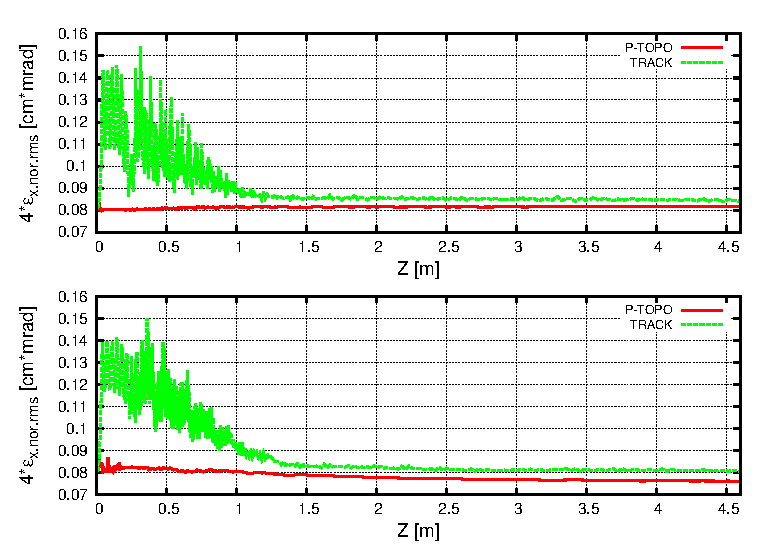
\includegraphics[width=\textwidth]{Img/ADS_RFQ_emit1.eps}
%        \caption{0mA(上)和15mA(下)时RFQ中的横向发射度}
%    \end{subfigure}
%    \begin{subfigure}[b]{0.9\textwidth}
%        \includegraphics[width=\textwidth]{Img/ADS_RFQ_emit2.eps}
%        \caption{0mA(上)和15mA(下)时RFQ中的纵向发射度}
%    \end{subfigure}
%    \caption{RFQ中的横向发射度和纵向发射度}\label{fig:ADS_RFQ_emit}
%\end{figure}

\begin{figure}[!htb]
    \centering
    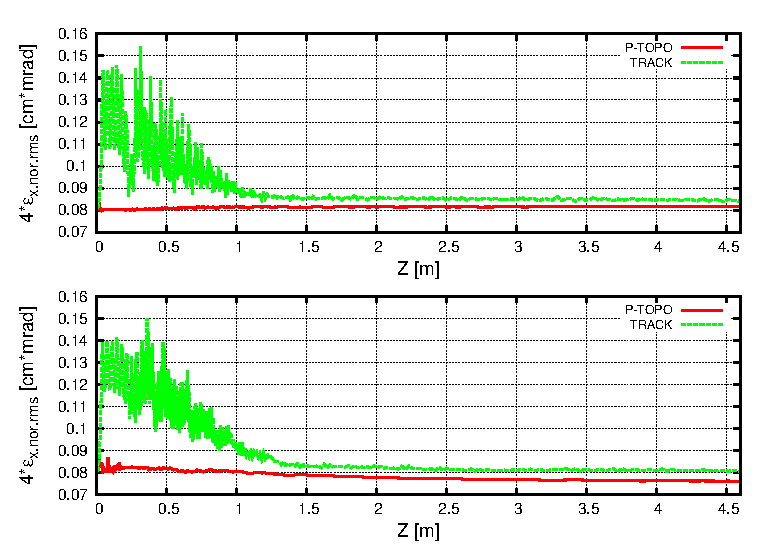
\includegraphics[width=0.9\textwidth]{Img/ADS_RFQ_emit1.eps}
    \caption{0mA(上)和15mA(下)的C-ADS注入器I的RFQ中的横向发射度变化}
    \label{fig:ADS_RFQ_emit_transverse}
\end{figure}
\begin{figure}[b]
    \centering
    \includegraphics[width=0.9\textwidth]{Img/ADS_RFQ_emit2.eps}
    \caption{0mA(上)和15mA(下)的C-ADS注入器I的RFQ中的纵向发射度变化}
    \label{fig:ADS_RFQ_emit_longitudinal}
\end{figure}


图\eqref{fig:ADS_RFQ_size1}是使用P-TOPO和TRACK在15mA下对RFQ模拟得到的横向束团尺寸演化,
图~\eqref{fig:ADS_RFQ_size2}是使用~P-TOPO 和 TRACK 在15mA下对RFQ模拟得到的纵向束团尺寸和能散演化,
其中红色实线为P-TOPO的结果而绿色虚线为TRACK的结果。
两个程序在束团均方根尺寸上吻合得很好,其差别在合理范围内。
通过P-TOPO模拟计算,我们认为C-ADS注入器I的RFQ设计能够有效的控制束团的发射度和尺寸。

\begin{figure}[!tbh]
    \centering
    \includegraphics[width=0.9\textwidth]{Img/ADS_RFQ_size1.eps}
    \caption{C-ADS注入器I的RFQ中束团横向均方根尺寸变化}
    \label{fig:ADS_RFQ_size1}
\end{figure}

\begin{figure}[!tbh]
    \centering
    \includegraphics[width=0.9\textwidth]{Img/ADS_RFQ_size2.eps}
    \caption{C-ADS注入器I的RFQ中束团纵向均方根尺寸和能散变化}
    \label{fig:ADS_RFQ_size2}
\end{figure}

\subsection{超导段模拟}  \label{section:ADS_simulation_SC}
在超导段中,聚束腔和加速腔的场由文件导入,P-TOPO使用数值插值来得到粒子所受到的场强。
在设计的15mA流强下,RFQ出口处3.2MeV的质子束流经过聚束,通过MEBT进入超导段,逐渐加速到10MeV。在超导段中我们使用P-TOPO和~TraceWin来进行模拟。

图\eqref{fig:ADS_SC_emit}为P-TOPO和TraceWin在15mA流强下对RFQ模拟得到的横向和纵向发射度演化,其中红色实线为P-TOPO的结果,而绿色虚线为TraceWin的结果。
两个程序得到的结果相一致。其中横向发射度除了在螺线管处有一个峰值外,基本保持不变。
螺线管处的峰值是一方面是因为发射度需要在共轭坐标下讨论, 而 PTOPO 和 TraceWin 在螺线管中的统计量并不是共轭量;
另一方面是因为在束团进入螺线管的时候相空间发生扭曲。
%P-TOPO和TraceWin都是以时间t为基本变量,即发射度是由同一时刻的粒子信息统计得到,
%而不是由同一纵向位置的粒子得到,因此,
%,部分粒子先进入,部分粒子还没有进入,导致
%,从而导致统计发射度的突变
束团的纵向发射度有略微增长,其增长幅度在20\%以内。
发射度增长是由空间电荷力、磁铁边缘场的非线性效应、以及超导腔内的非线性纵向力导致,
这几个来源共同驱动发射度增长,并使粒子相空间扭曲,最终会导致束晕的产生。
P-TOPO的模拟中,出口能量为10.01MeV,而TraceWin的模拟出口能量为10.06MeV。
\begin{figure}[!htb]
    \centering
    \begin{subfigure}[b]{0.9\textwidth}
        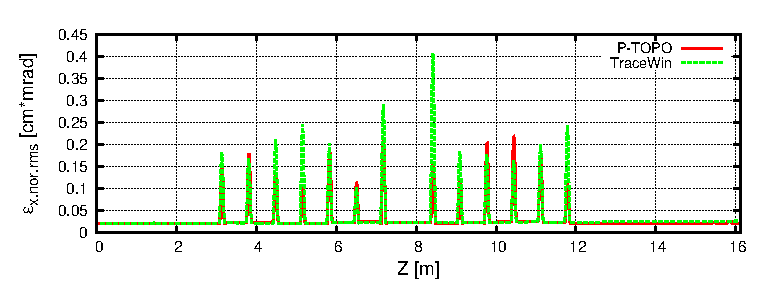
\includegraphics[width=\textwidth]{Img/ADS_SC_emit1.eps}
        %\caption{}
    \end{subfigure}
    \begin{subfigure}[b]{0.9\textwidth}
        \includegraphics[width=\textwidth]{Img/ADS_SC_emit2.eps}
        %\caption{}
    \end{subfigure}
    \caption{C-ADS注入器I的超导段横向发射度和纵向发射度变化}\label{fig:ADS_SC_emit}
\end{figure}

图\eqref{fig:ADS_SC_size}是P-TOPO和TraceWin在15mA下对超导段模拟得到的横纵向束团尺寸和能散,
其中红色实线为P-TOPO的结果而绿色虚线为TraceWin的结果。
两个程序模拟结果的细微差别来自于两个程序获取同步相位的方法不同。
TraceWin使用时间漂移法获得同步相位,而P-TOPO使用扫相获得同步相位。
束团的横向尺寸相比管道半径都很小,而纵向尺寸也被聚束腔和接下来的各个加速腔有效地压缩,在这种情况下束损通常不会大量形成。
\begin{figure}[!htb]
    \centering
    \begin{subfigure}[b]{0.9\textwidth}
        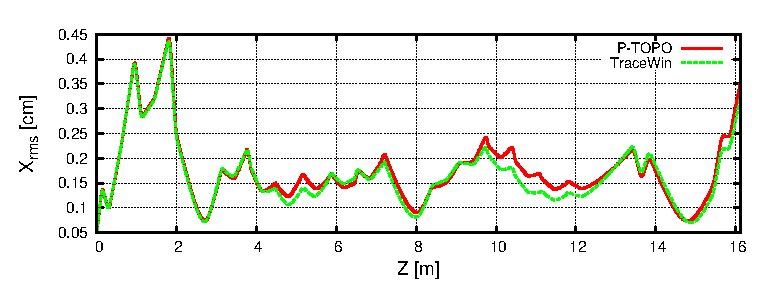
\includegraphics[width=\textwidth]{Img/ADS_SC_size1.eps}
        %\caption{}
    \end{subfigure}
    \begin{subfigure}[b]{0.9\textwidth}
        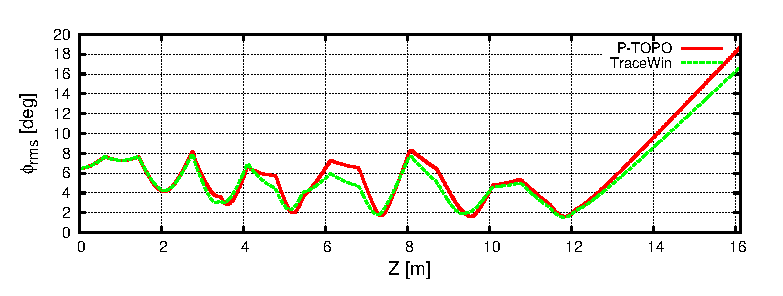
\includegraphics[width=\textwidth]{Img/ADS_SC_size2.eps}
        %\caption{}
    \end{subfigure}
    \begin{subfigure}[b]{0.9\textwidth}
        \includegraphics[width=\textwidth]{Img/ADS_SC_size3.eps}
        %\caption{}
    \end{subfigure}
    \caption{C-ADS注入器I的超导段束团横纵向尺寸以及能散变化}\label{fig:ADS_SC_size}
\end{figure}

\subsection{总结}  \label{section:ADS_simulation_conclusion}

通过使用P-TOPO对C-ADS注入器I进行模拟,我们一方面验证了注入器I设计的合理性,另一方面也通过和其他模拟程序的对比验证了P-TOPO的正确性。

模拟结果表明,C-ADS注入器I能够有效的对粒子束团进行加速。
无论是在零流强还是在15mA流强下,粒子在RFQ和超导段中的传输效率都在99.9\%以上,
而且束团尺寸和束损都得到了有效控制,横向和纵向的发射度都保持良好。

我们还将P-TOPO的模拟结果与其他模拟程序的结果进行了对比,
不同程序的结果基本吻合,其差别在合理范围之内,P-TOPO的正确性得到了验证。
%微小的差别主要是因为空间电荷力的计算方式以及统计数据的方式不同。
%特别是P-TOPO是以时间t为基本变量,而TRACK是以位置z为基本变量,
%因此粒子信息收集、空间电荷力的计算、以及粒子推动方式都有微小的差别。

\section{三阶共振模拟}            \label{section:3rd_order_simulation}
我们使用Symplectic算法在周期聚焦结构中进行粒子跟踪和模拟,来研究束流中的三阶共振现象。
如果使零流强的周期相移为86.3259度,并将10个周期视为一个环,则环的工作点为2.3979。
随着流强的增加,相移会被压缩,工作点会在0.6A左右穿过2.3333的三阶共振线。
如果环中存在一个六极磁铁,则束流会出现明显的三阶共振现象。

图\eqref{fig:emitGrowthCompare}为六极铁$K=1.0$时不同流强下的束流发射度增长变化。
可以看到,束流发射度在流强为 0.1A 和 0.2A 时基本保持不变,这时的工作点约为2.40。
但是发射度在流强为0.4A, 0.6A, 和0.8A时持续增长,这时的工作点在2.3333附近,可知其发射度增长是由于三阶共振导致。

\begin{figure}[!htb]
    \centering
    \includegraphics[width=0.95\textwidth]{Img/SymplecticEmitGrowthCompare.pdf}
    \caption{不同流强下的发射度增长}
    \label{fig:emitGrowthCompare}
\end{figure}

图\eqref{fig:Poincare}是工作点为2.3333附近时的粒子坐标的庞加莱截面,
其中颜色越暗表示粒子密度越大,而不同的图片代表粒子处于不同的初始位置。
受空间电荷效应驱动,庞加莱截面会被被扭曲,并塑造成三角形形状。
受到三阶共振影响的粒子的横向位置会逐渐变大。

\begin{figure}[!htb]
    \centering
    \begin{subfigure}[b]{0.48\textwidth}
        \includegraphics[width=\textwidth]{Img/particle_contour_nlevel9/sptc00002_xpx.pdf}
        \caption{}
    \end{subfigure}
    \begin{subfigure}[b]{0.48\textwidth}
        \includegraphics[width=\textwidth]{Img/particle_contour_nlevel9/sptc00005_xpx.pdf}
        \caption{}
    \end{subfigure}
    \begin{subfigure}[b]{0.48\textwidth}
        \includegraphics[width=\textwidth]{Img/particle_contour_nlevel9/sptc00003_xpx.pdf}
        \caption{}
    \end{subfigure}
    \begin{subfigure}[b]{0.48\textwidth}
        \includegraphics[width=\textwidth]{Img/particle_contour_nlevel9/sptc00006_xpx.pdf}
        \caption{}
    \end{subfigure}
    \caption{三阶共振附近的庞加莱截面}\label{fig:Poincare}
\end{figure}
本次模拟的三阶共振效应小,因此导致的发射度增长很小。
这个小的增长效应需要较高精度的模拟。
正是因为Symplectic算法在长程研究中几乎不出现非自然的发射度增长,其精确度较高,
所以本次模拟中微小的发射度增长才能较为明显的通过模拟得到。

\section{共振穿越研究}            \label{section:Resonance_crossing}
在一个实际的加速器中,特别是直线加速器中,
外部元件的聚焦强度一般随着束流被加速而逐渐变化,
束流的周期相移也随之变化。
在这个过程中,束流有可能穿越结构共振禁带,即“共振穿越”。

加速中由各种非线性驱动的共振被认为是导致束流恶化的主要来源,例如束流发射度增长、束晕、束损等。
除了加速器元件产生的非线性效应之外,束团内部的空间电荷效应也是非线性共振的一个来源。
在强流质子加速器中,空间电荷效应会在不同自由度之间产生耦合,
相关学者已经在数值和实验上对此进行了很多研究~\cite{accelerator2013chao,accelerator2004lee,reiser2008theory}。
但是对于束流在穿越过程中具体如何演化,以及不同穿越速度对于束流有什么影响,人们并没有一个统一的结论。
如果共振穿越无法避免,目前人们对于如何处理共振穿越仍然存在这样的争议:是应该尽量绝热变化以达到更好的匹配,还是应该尽快完成穿越以减少束流在共振区的时间?

这些问题在加速器设计中非常重要。
为了探寻这些问题,我们基于前人对结构共振的研究,
对束流穿过结构共振禁带时的一些现象进行了模拟研究,
比如束流和粒子的相干和非相干特性将如何演化、
束流如何自发地受到结构共振的影响、
以及不同穿越速度对于束流发射度的影响等。

%节\eqref{section:Crossing_introduction}对共振穿越问题的一些背景进行了介绍;
接下来,节\eqref{section:Crossing_model}将简要介绍了结构共振的模型,并定义了用来描述相干和非相干效应的一些术语;
节\eqref{section:Crossing_Coherent}中给出了禁带的方程,使用多粒子PIC追踪程序模拟了束流穿越相干结构共振时的现象,并在暂态意义上进行了讨论;
节\eqref{section:Crossing_Incoherent}讨论了非相干共振的粒子特征;
最后节\eqref{section:Crossing_Summary}进行了总结。

%\subsection{简介}
%\label{section:Crossing_introduction}


\subsection{物理模型}
\label{section:Crossing_model}
束流运动的表述有两个层面,每个层面分别都有对应的模型来描述。
其非线性共振的两个层面的模型分别为单粒子动力学(非相干效应)和RMS束流动力学(相干效应)。
单粒子动力学描述的一个典型例子是共振线图中由于加速器中多级铁和Lattice的误差导致的各阶共振线$n\nu_x+m\nu_y$。
共振线图被广泛应用在加速器的工作点选择和实际运行中。
考虑到非线性效应,加速器的工作点会产生偏移~\cite{fedotov2001space},
所以当束流工作点靠近共振线时就会发生单粒子周期共振穿越~\cite{franchetti2006particle}。
对于RMS束流动力学描述,外部元件和内部空间电荷效应产生的非线性效应在束流集体不稳定性中起到了非常关键的作用
\cite{sacherer1968transverse, sacherer1973longitudinal},
其可以通过以自洽的方式求解扰动的弗拉索夫方程来描述\cite{chao1993physics,gluckstern1970oscillation,gluckstern1970stability}。
然而,虽然人们付出了极大地努力来扩展这些模型以涵盖各种束流条件,但是可解决的问题只是局限于某些特定的情况。

对于强流离子束流中的空间电荷效应导致的集体不稳定性,其研究一方面从RMS包络方程出发~\cite{sacherer1971rms},
其中二阶不稳定性,即束流包络不稳定性,得到了人们广泛而深入的研究 ~\cite{14,15,li2014envelope,li2015space,21,22}。
而另一方面的研究从自洽的求解弗拉索夫-泊松方程出发 ~\cite{11,li2018structure,18,19}。
研究表明,求解弗拉索夫-泊松方程得到的二阶偶共振正是包络方程的得到的相干共振。
最近研究提出了一种空间电荷物理中的弗拉索夫-泊松模型的通用理论~\cite{11,li2018structure},
预测了在Lattice参数没有被精心优化的情况下,结构共振会伴随构造本征模式发生,
另外,低阶的结构共振禁带可以自然的作为高阶结构共振禁带的一部分\footnote{数学证明详见参考文献~\cite{li2018structure}}。

作为对弗拉索夫-泊松模型的理论研究的延伸,我们选取了$90^{\circ}$相移附近的二阶共振禁带进行研究,并使用PIC模拟来验证了理论预测的有效性。这些研究可以很容易地扩展到更高阶的模式,比如三阶($60^{\circ}$)和六阶结构共振($120^{\circ}$)~\cite{36,40}。
需要注意的是,束流和结构共振之间的相互作用必须在瞬态状态下进行研究。
而低阶模是高阶模的组成部分这一概念是理解模拟和实验结果的关键~\cite{groening2009experimental,33}。

本节简要介绍了结构共振的物理模型和基本的处理方法,其中可解的耦合弗拉索夫-泊松方程仅限于4D KV分布~\cite{20}。
一般来说,对束流动力学行为的研究是在哈密顿系统的框架中进行的,
而粒子哈密顿系统中不可积的部分可以被视为微扰,这样共振条件就可以使用微扰理论来得到。
接下来,我们使用周期性的FODO结构来模拟加速器中的连续束的演变, 考虑到周期聚焦结构中完全匹配的束流的哈密顿量是恒定的,平衡分布函数和对应的哈密顿量可以表示为:
\begin{eqnarray}\label{eq2.1}
  f_0(x,p_x,y,p_y) =f(H_0),  \quad  H_0&=&k_x(s)x^2+p_x^2+k_y(s)y^2+p_y^2+V_{sc}(x,y)\text{。}
\end{eqnarray}
其中 $k_x(s)$和$k_y(s)$外部四极铁的聚焦强度, $V_{sc}(x,y)$是空间电荷势。分布函数 $f_0$必须同时满足Vlasov方程和 Poisson方程:
\begin{eqnarray}\label{eq2.2}
\frac{\partial f_0}{\partial s} + [f_0,H_0]=0,   \quad \Delta V_{sc}(x,y)  = \frac{1}{\epsilon_0}  \int \int f_0 dxdy,
\end{eqnarray}
其中 $[,]$为泊松括号。

如果粒子分布函数存在一个扰动 $f_1$,其将会导致空间电荷势受到扰动$V_1=H_1$。扰动后的弗拉索夫方程和泊松方程可以表示为:
\begin{eqnarray}\label{eq2.3}
\frac{\partial f_1}{\partial s} + [f_1,H_0] +  [f_0,V_1]=0,   \quad \Delta V_1(x,y)  = \frac{1}{\epsilon_0}  \int \int f_1 dxdy\text{。}
\end{eqnarray}
目前认为,这组方程只有在粒子分布为理想的KV分布$f_0=\delta(H_0)$的时候才可解。一般情况下,束流内受扰动的空间电荷势可以表示为多项式的形式:
\begin{eqnarray}\label{eq2.4}
V_1=\sum_{m=0}^{n}A_m(s)x^{n-m}y^m +\sum_{m=0}^{n-2}A_m^{(1)}(s)x^{n-m}y^m+\cdots\text{。}
\end{eqnarray}
集体模$I_{j;k,l}(s)$可以在适当的边界条件下得到。
对于式~\eqref{eq2.4}中的$n$阶偶数模和奇数模可以根据$m$是偶数或奇数来分开处理,
其直接代表了粒子分布在扰动后在实空间中的倾角。设 $S$为一个聚焦周期的长度,
$I_{j;k,l}(s)$ 将满足$\mathbf{I}'(s) = \mathbf{M}(S)\mathbf{I}(s)$,这正是$Mathieu$方程。
而这个系统的稳定性将由其雅克比矩阵$M(S)$的本征值$\lambda$决定,详细的数学证明见参考文献~\cite{11,li2018structure,18,19}。

根据之前的研究\cite{11,li2018structure},结构共振条件可以显式的表达为$\Phi_{j;k,l}+\Phi_{j;k,l}=n\times 360^{\circ}$和$\Phi_{j;k,l}/\Phi_{e}=n/m$,其中$\Phi_{j;k,l}$为集体模$I_{j;k,l}$的本征相位;$\Phi_{e}$是一个周期中的包络振荡相移,恒为$360^{\circ}$。结构共振会随着本征相位锁定的现象发生,而发生结构共振的参数空间被称为不稳定禁带。

\subsection{结构共振穿越 -- 相干效应}
\label{section:Crossing_Coherent}
在加速器设计与运行中有一条经验准则:“如果共振穿越不可避免,则穿越速度应该越快越好。”
比如在一些直线加速器的设计中,一开始的零流强相移大于$90^{\circ}$,之后在几个周期之内迅速降到 $90^{\circ}$以下。
接下来,我们使用$90^{\circ}$相移附近的二阶结构共振来研究当穿越共振禁带时的束流和结构共振之间的相互作用
\footnote{如上文说述,二阶集体模实际上是四阶集体模的一部分~\cite{li2018structure},所以在下文中二阶模指的是二阶/四阶混合禁带。}。
为了简化,我们使束流在两个方向上的发射度相等,并使用对称的周期FODO聚焦结构($|k_x|=|k_y|$)。

\subsubsection{二阶相干效应}
对于二阶偶数模,束流内部的扰动的空间电荷势为  $V_{2e} = A_0(s)x^2 + A_2(s)y^2$;
对于二阶奇数模,其为 $V_{2o}=A_1(s)xy$。
通过动力学系统 $\mathbf{I}'(s)=\mathbf{M}(s)\mathbf{I}(s)$ 可以得到 $({I}_{0;2,0}, I_{2;0,2})$ 和  $(I_{1;1,1}, I_{1;1,-1})$ ,
分别代表二阶偶数模和奇数模~\cite{11, li2018structure, 18},其雅克比矩阵$\mathbf{M}(s)$可以表示为:
\begin{eqnarray}\label{eq2.5}
\mathbf{M}(s)=
\left(
  \begin{array}{cccc}
    0         & 1         & 0         & 0         \\
    J_{21}(s) & J_{22}(s) & J_{23}(s) & 0         \\
    0         & 0         & 0         & 1         \\
    J_{41}(s) & 0         & J_{43}(s) & J_{44}(s) \\
  \end{array}
\right),
\end{eqnarray}
上式中每个元素$J_{ij}(s)$的显式表达见附录~\eqref{appdendix:Jacobi}.

\begin{figure}
    \centering
    \begin{subfigure}[b]{0.48\textwidth}
        \includegraphics[width=\textwidth]{Img/evenDepressedAbs.pdf}
        \caption{}
        \label{sfig:stopbandEvenAbs}
    \end{subfigure}
    \begin{subfigure}[b]{0.48\textwidth}
        \includegraphics[width=\textwidth]{Img/oddDepressedAbs.pdf}
        \caption{}
        \label{sfig:stopbandOddAbs}
    \end{subfigure}

    \begin{subfigure}[b]{0.48\textwidth}
        \includegraphics[width=\textwidth]{Img/evenDepressedArg.pdf}
        \caption{}
        \label{sfig:stopbandEvenArg}
    \end{subfigure}
    \begin{subfigure}[b]{0.48\textwidth}
        \includegraphics[width=\textwidth]{Img/oddDepressedArg.pdf}
        \caption{}
        \label{sfig:stopbandOddArg}
    \end{subfigure}
    \caption{二阶偶数模和奇数模的本征值 $Abs[\lambda_{j;k,l}]$ 和本征相位 $\Phi_{j;k,l}$ 随考虑空间电荷效应后的相移 $\sigma$ 的变化}
    \label{fig:stopband}
\end{figure}

从包络方程出发的包络不稳定性已经得到了大量的研究,其描述了和二阶偶数模相同的物理机制~\cite{11,li2018structure,18}。
最近,人们使用Chernin模型研究了“和共振”与“差共振”不稳定性~\cite{21,22},研究给出了与从二阶偶模结构共振出发相同的结果。
GSI和CERN的研究人员也在实验上对 $I_{0;2,0}$ 和 $I_{2;0,2}$ 进行了测量~\cite{singh2014observations,cernAdrian}。
图~\eqref{fig:stopband} 是在流强不变而考虑空间电荷效应后的相移$\sigma$从 $95^{\circ}$
变化到 $75^{\circ}$ 时的二阶偶数模与奇数模的本征值 $Abs[\lambda_{j;k,l}]$ 和本征相位 $\Phi_{j;k,l}$ 的变化
\footnote{我们使用了对称束流条件,因此无论考虑空间电荷效应与否,两个自由度上的相移都相等。},
其对应的的零流强相移 $\sigma_0$ 从 $110^{\circ}$ 变化到 $80^{\circ}$。
如图所示,对于二阶偶数模,每当本征相位合流时,比如 $84^\circ \sim 89^\circ$~(本征相位
发生锁定 $\Phi_{2;0,2}=\Phi_{0;2,0}$, 也被叫做合流共振~\cite{li2018structure}), 本征值$Abs[\lambda]$ 就
会离开单位圆,其绝对值会离开$1.0$,这代表了集体不稳定性,会导致发射度增长。
因为这里选择了对称束流条件,二阶奇数模不会导致任何不稳定性。
下面,我们在PIC模拟~\cite{23,24}中使用由400个聚焦强度线性变化的FODO周期构成的 Lattice,以研究结构共振穿越。
初始分布采用水袋分布,宏粒子数为50000。


\subsubsection{二阶结构共振穿越研究}

在束流流强固定,而外部四极铁的聚焦强度逐渐变化的条件下,我们对束流穿越二阶结构共振禁带从两个方面进行了研究。
一方面使束流周期相移从小到大变化(从下向上穿越,即周期相移 $\sigma$在400个周期里线性地从$75^{\circ}$ 增加到 $95^{\circ}$);
另一方面正相反,使束流周期相移从大到小变化(从上向下穿越)。

图~\eqref{fig:phase_advance} 显示了束流相位从下方和从上方分别穿越结构共振禁带的情况,其中灰色区域为共振禁带,大约为 $84^ {\circ}<\sigma<89^{\circ}$。蓝色和红色曲线分别代表模拟得到的X和Y方向的周期相移演化,而黑色曲线代表平滑处理后的平均周期相移。
原则上,模拟的周期相移被限制在黄色和绿色线所界定的区域内,黄色和绿色直线分别是预期的零流强周期相移和考虑空间电荷效应后的周期相移。
垂直的黑色直线为束流实际进入和穿出共振禁带的位置,绿色直线和黑色曲线与禁带边界之间的交叉点分别表示束流在设计上和实际模拟中进入和穿出共振禁带的位置。
图~\eqref{fig:emittance}为相应的rms发射度的变化,图~\eqref{fig:phase_advance}相同,垂直的黑色直线表示束流进入和穿出共振禁带时的位置。

在图~\eqref{sfig:75_95phase}中当束流从下方穿越共振区时,模拟得到的周期相移一开始与预期值相符并单调增加,但是当束流在大约200周期进入禁带后,束流周期相移穿越的速度开始变得比预期要快(如绿色直线和黑色曲线分别与禁带边界之间的交叉点所示),束流在大约250个周期时就穿出了共振禁带,并到达了一个局部平衡态。
图~\eqref{sfig:75_95emittance}显示束流一旦进入结构共振禁带,其rms发射度就开始增长,而在束流穿越禁带之后,发射度就停止增长,其中物理机制会在下文中详细讨论。

相反的,图~\eqref{sfig:95_75phase}和图~\eqref{sfig:95_75emittance}显示了从上方穿越共振禁带时的周期相移和发射度的变化。在图~\eqref{sfig:95_75phase}中,可以明显看出束流比预期在禁带里停留的时间更长,即束流穿越共振带的速度更慢,在大约370个周期后才离开共振带。而且同从下方穿越的情况相比,束流的发射度增长更多。

\begin{figure}[thbp]
    \centering
    \begin{subfigure}[b]{0.48\textwidth}
        \centering
        \includegraphics[width=\textwidth]{Img/75_95_PhaseAdvance.pdf}
        \caption{}
        \label{sfig:75_95phase}
    \end{subfigure}
    \begin{subfigure}[b]{0.48\textwidth}
        \centering
        \includegraphics[width=\textwidth]{Img/95_75_PhaseAdvance.pdf}
        \caption{}
        \label{sfig:95_75phase}
    \end{subfigure}
    \caption{从下方穿越共振区(左)与从上方穿越共振区(右)的周期相移比较}
    \label{fig:phase_advance}
\end{figure}

\begin{figure}[thbp]
    \centering
    \begin{subfigure}[b]{0.48\textwidth}
        \centering
        \includegraphics[width=\textwidth]{Img/75_95_Emittance.pdf}
        \caption{}
        \label{sfig:75_95emittance}
    \end{subfigure}
    \begin{subfigure}[b]{0.48\textwidth}
        \centering
        \includegraphics[width=\textwidth]{Img/95_75_Emittance.pdf}
        \caption{}
        \label{sfig:95_75emittance}
    \end{subfigure}
    \caption{从下方穿越共振区(左)与从上方穿越共振区(右)的发射度增长率($\epsilon_f/\epsilon_i$)比较
     }
    \label{fig:emittance}
\end{figure}

共振穿越必须在瞬态的意义上进行研究~\cite{li2018structure}。实际上,共振禁带的上边界和下边界随着穿越中的束流发射度增长也发生了变化。
在从下方穿越的情况下,禁带的上边界移动到了大约 $90^{\circ}$ 附近,束流也在禁带里多停留了15个周期,直到265个周期才穿出禁带。
同样的,对于从上方穿越的情况,禁带的下边界也略微向上移动,束流比预期中更早地(大约在300个周期左右)就穿出了禁带。
这两种情况的一个特性就是共振穿越的速度不同。当束流从下向上穿越时,共振禁带会有一个“吸引”效应;而当束流从上向下穿越时,共振禁带会有一个“排斥”效应。其原因在于,在一般意义上,在外部场和内部空间电荷场的综合影响下,
如果束流发生任何“不稳定”,比如rms发射度增长或者产生束晕,束流总是自发去摆脱这种不平衡。
从能量的观点来看,束流总是倾向于“释放”能量,以到达一个能量最低的平衡态。因此很自然的,束流总是倾向于使空间电荷势减弱~\cite{li2014envelope}。
研究表明一旦束流受到结构共振的影响,瞬态束流周期相移压缩因子$\eta=\sigma/\sigma_0$会变得大于设计值,这一结果符合上文的理论。

\begin{figure}
    \centering
    \begin{subfigure}[b]{0.24\textwidth}
        \includegraphics[width=\textwidth]{Img/7595Ptc050.pdf}
        \caption{}
        \label{sfig:75_95_ptc1}
    \end{subfigure}
    \begin{subfigure}[b]{0.24\textwidth}
        \includegraphics[width=\textwidth]{Img/7595Ptc150.pdf}
        \caption{}
        \label{sfig:75_95_ptc2}
    \end{subfigure}
    \begin{subfigure}[b]{0.24\textwidth}
        \includegraphics[width=\textwidth]{Img/7595Ptc250.pdf}
        \caption{}
        \label{sfig:75_95_ptc3}
    \end{subfigure}
    \begin{subfigure}[b]{0.24\textwidth}
        \includegraphics[width=\textwidth]{Img/7595Ptc350.pdf}
        \caption{}
        \label{sfig:75_95_ptc4}
    \end{subfigure}

    \begin{subfigure}[b]{0.24\textwidth}
        \includegraphics[width=\textwidth]{Img/9575Ptc050.pdf}
        \caption{}
        \label{sfig:95_75_ptc1}
    \end{subfigure}
    \begin{subfigure}[b]{0.24\textwidth}
        \includegraphics[width=\textwidth]{Img/9575Ptc150.pdf}
        \caption{}
        \label{sfig:95_75_ptc2}
    \end{subfigure}
    \begin{subfigure}[b]{0.24\textwidth}
        \includegraphics[width=\textwidth]{Img/9575Ptc250.pdf}
        \caption{}
        \label{sfig:95_75_ptc3}
    \end{subfigure}
    \begin{subfigure}[b]{0.24\textwidth}
        \includegraphics[width=\textwidth]{Img/9575Ptc350.pdf}
        \caption{}
        \label{sfig:95_75_ptc4}
    \end{subfigure}
    \caption{从下方穿越共振区(上)与从上方穿越共振区(下)的穿越过程中的粒子相空间形状$(x-p_x)$}
    \label{fig:95_75_ptc}
\end{figure}

图~\eqref{fig:95_75_ptc}显示了从下方穿越共振区(上)与从上方穿越共振区(下)的穿越过程中在不同的FODO周期位置处的粒子分布相空间,
图中的位置分别在第50、150、250、350个周期处。从图中可以清楚地看到,无论是从下方还是从上方穿越结构共振禁带,
束流一进入共振禁带,相空间就出现了四个共振岛的结构,这正是四阶结构共振的现象。
四阶结构共振会出现在二阶结构共振禁带的原因为低阶禁带是高阶结构共振禁带的一部分~\cite{11,li2018structure}。一般来说,不同阶的结构共振的出现需要合适的驱动力(式~\eqref{eq2.4})。
从WB初始分布开始,二阶和四阶扰动势从一开始就存在,并不断演变。
因此,在二阶结构共振禁带中的相空间本就应该既出现双重结构又有四重结构 (我们将会在第~\eqref{section:Crossing_Incoherent}节中给出一个例子)。
最后,由于这些混合的结构共振效应,束流产生了束晕。

\subsubsection{结构共振穿越速度和rms发射度增长}
%FFAG中的单粒子运动表明共振穿越必须被仔细地研究~\cite{26}。
为了研究如何处理共振穿越这个问题,这里我们主要关注束流的均方根发射度与结构共振穿越速度之间的关系。
与上一小节中处理束流周期相移的方法相似,在这里,我们一使用400个FODO周期,其中前$N$个周期($N$=10, 20, 50, 100, 200, 400)的束流周期相移线性的从$75^\circ$增加到  $95^\circ$(从下方穿越)或者从$95^\circ$ 减小到 $75^\circ$(从上方穿越),
并使用400个周期后最终的rms发射度增长作为评价束流品质的标准。

图~\eqref{sfig:CrossingSpeed_byStopband1}为最终发射度增长和渐变周期数$N$的关系。在相同的共振穿越速度下,从上方穿越的发射度增长远大于从下方穿越的发射度增长,这表明了和我们在图~\eqref{fig:emittance}中解释的相同的物理机制。
对于不同的共振穿越速度,从上方穿越和从下方穿越都表明束流应尽可能快地穿越结构共振禁带,以避免显著的发射度增长。
图~\eqref{sfig:CrossingSpeed_byStopband2}为发射度增长和束流在共振禁带内的周期数的关系,
发射度增长与束流停留在结构共振禁带中的时间几乎线性相关。

\begin{figure}[thbp]
    \centering
    \begin{subfigure}[b]{0.48\textwidth}
        \includegraphics[width=\textwidth]{Img/EmittanceGrowth.pdf}
        \caption{}
        \label{sfig:CrossingSpeed_byStopband1}
    \end{subfigure}
    \begin{subfigure}[b]{0.48\textwidth}
        \includegraphics[width=\textwidth]{Img/EmittanceGrowthByStopband.pdf}
        \caption{}
        \label{sfig:CrossingSpeed_byStopband2}
    \end{subfigure}
    \caption{
    a): 400个FODO周期后的最终发射度增长率与用于共振跨越控制的~FODO周期数的关系;
    b): 400个FODO周期后的最终发射度增长率与束流在结构共振禁带中的有效周期数的关系。}
    \label{fig:CrossingSpeed}
\end{figure}

\subsection{单粒子动力学 -- 非相干效应}
\label{section:Crossing_Incoherent}
从非相干单粒子动力学的角度来看,因为之前所讨论的周期相移主要在$\sigma\sim90^\circ$附近,
人们很直观的会将4重结构共振归因于4阶particle-core共振($90^\circ/360^\circ=1:4$)
\footnote{$360^\circ$在这里用来表示束核的振荡频率,即在一个FODO周期中完全匹配束流的束核振荡一次。}。
因此,结构共振穿越过程中的particle-core共振岛向核心运动或向外运动的方向被用来解释所形成的四重相空间结构以及当结构共振从下方和上方穿越时束晕的严重差异~\cite{25} 。

图~\eqref{fig:TestPtc}为使用particle-core共振模型的单粒子在相空间中的Poincar\'{e}截面~\cite{27,li2015space}。
很显然,当从上方穿越结构共振禁带时,通过分叉过程~\cite{29,li2016nonlinear}在原点产生四个particle-core 共振岛,并在穿越过程中逐渐向外移动
(图~\eqref{sfig:TestPtc1} $\rightarrow$ 图~\eqref{sfig:TestPtc4});
相反的,当从下方穿越时,particle-core 共振岛从外向核内移动
(图~\eqref{sfig:TestPtc4} $\rightarrow$ 图~\eqref{sfig:TestPtc1})。
人们直观上会认为相空间中的四重结构与这种particle-core共振有关。
一方面因为这种particle-core 共振在这种共振图像中可以逐渐将核心中的粒子带到外部并形成稳定的四重相空间结构;
另一方面因为如果particle-core 共振岛从外部朝向内核移动,由于最初外部没有粒子,较少的粒子会占据四重共振岛并且生成更少的束晕。
在目前的理解下这个图像可能会产生束晕,但是我们的研究认为这个图像并不对束晕的产生起主导作用。
然而,这是不对的,因为如果空间电荷效应是束流系统中唯一的非线性效应,则$N$重共振岛结构主要取决于相干集体效应,而不是非相干 particle-core共振。
例如,非相干的四阶particle-core共振不能预测模拟中从下方穿越和从上方穿越都出现的相空间中的两个共振岛结构,
如图~\eqref{fig:Ptc2tail}所示,而这正是二阶结构共振(相干效应)的证据。
正如之前的研究~\cite{li2014envelope}所指出的,我们认为,非相干 particle-core共振仅在长时间尺度上可能导致四重相空间结构。
在这里,我们认为在模拟中形成的四重相空间结构对应于二阶/四阶混合相干结构共振。

\begin{figure}
    \centering
    \begin{subfigure}[b]{0.24\textwidth}
        \includegraphics[width=\textwidth]{Img/TestParticle1.pdf}
        \caption{}\label{sfig:TestPtc1}
    \end{subfigure}
    \begin{subfigure}[b]{0.24\textwidth}
        \includegraphics[width=\textwidth]{Img/TestParticle2.pdf}
        \caption{}\label{sfig:TestPtc2}
    \end{subfigure}
    \begin{subfigure}[b]{0.24\textwidth}
        \includegraphics[width=\textwidth]{Img/TestParticle3.pdf}
        \caption{}\label{sfig:TestPtc3}
    \end{subfigure}
    \begin{subfigure}[b]{0.24\textwidth}
        \includegraphics[width=\textwidth]{Img/TestParticle4.pdf}
        \caption{}\label{sfig:TestPtc4}
    \end{subfigure}
    \caption{使用粒子束核模型得到的单粒子Poincar\'{e}截面}
    \label{fig:TestPtc}
\end{figure}

\begin{figure}[!hbp]
    \centering
    \begin{subfigure}[b]{0.45\textwidth}
        \includegraphics[width=\textwidth]{Img/7595Ptc002050.pdf}
        \caption{从下向上穿越,205周期附近}
        \label{sfig:Ptc2tails1}
    \end{subfigure}
    \begin{subfigure}[b]{0.45\textwidth}
        \includegraphics[width=\textwidth]{Img/9575Ptc001800.pdf}
        \caption{从上向下穿越,180周期附近}
        \label{sfig:Ptc2tails2}
    \end{subfigure}
    \caption{相空间分布上的两个共振岛结构示意图}
    \label{fig:Ptc2tail}
\end{figure}


\subsection{总结}
\label{section:Crossing_Summary}

我们的研究清楚地揭示了束流穿越结构共振禁带时的瞬态行为。二阶/四阶混合相干结构共振对PIC模拟得到的结果给出了相当合理的解释。
必须再次强调的是,束流和结构共振之间的相互作用需要在瞬态的意义上进行研究。
由于束流的均方根特性被结构共振所改变,共振禁带的“吸引”和“排斥”效应是束流的一种自发反应。
研究还发现,束流的发射度增长几乎与束流受到结构共振影响的时间正相关。
束流的最终平衡态是结构共振和非线性阻尼的综合结果。
非相干particle-core共振可能造成粒子相位空间扭曲、发射度增长、或形成束晕,但其需要一个较长的时间尺度。

另一方面,我们的模拟清楚地证明了之前的理论预测,即低阶禁带自然地包含在高阶禁带中。
相同的理解还可以扩展到关于高阶结构共振的研究。
例如在 $60^{\circ}$周期相移附近($3 \times 60^{\circ} = 180^{\circ}$, $6 \times 60^{\circ} = 360^{\circ}$)~\cite{li2015space}和 $120^{\circ}$周期相移附近($3 \times 120^{\circ} = 360^{\circ}$, $6 \times 120^{\circ} = 720^{\circ}$)~\cite{11,36}
的三阶/六阶混合结构共振。
而对与空间电荷相关的相干和非相干共振的理解能够让我们更好地理解最近的实验结果~\cite{31,32,33}。
然而,尽管对非线性现象的解释有了一定进展,但是理论、数值模拟、和实验结果之间仍然存在着很大的距离。
在今后的研究中,我们还需要对实际的6D粒子动力学做进一步的研究。

\section{小结}                    \label{section:Simulation_conclusion}
首先,我们使用P-TOPO程序对C-ADS注入器I的RFQ和超导段分别进行了模拟,并且与其他程序进行了比较。
模拟结果证明了现有设计的合理性,束团的尺寸和发射度都得到了有效控制,束损以及能散也在合理范围之内,完全满足需求。
P-TOPO模拟结果其他程序结果的比较也验证了P-TOPO的正确性。

之后,我们在周期性聚焦结构中使用Symplectic算法进行了一个由于加速器元件和空间电荷效应导致的三阶共振模拟。
当工作点远离共振线时,束流不会出现发射度增长,而当其接近共振线时发射度会持续增长。

最后,我们使用P-TOPO程序对加速器中的共振穿越进行了研究。
研究清楚地揭示了束流穿越结构共振禁带时的瞬态行为。
研究也表明束流的发射度增长与束流受到结构共振影响的时间正相关。

将来我们将继续对P-TOPO进行拓展并加入更多新的功能,以满足强流加速器的各种需求,并实际的粒子动力学的研究做进一步的研究。